% \part{Template}\label{part:appendices}
\chapter{Network node ingredient lists}\label{ch:ingredients}

% the hierarchy is 
% chapter,section,subsection,etc

% todo: put the ingredient list pdf(s) here. they are on the wiki but need updating. I think the powerpoint lives on the Coffee lab PC but i may have slacked it to myself.

Below, there are ``ingredient lists" for key sections of the network experiment apparatus, including the optical chip.

\newpage

\begin{sidewaysfigure}[!t]
    \centering
    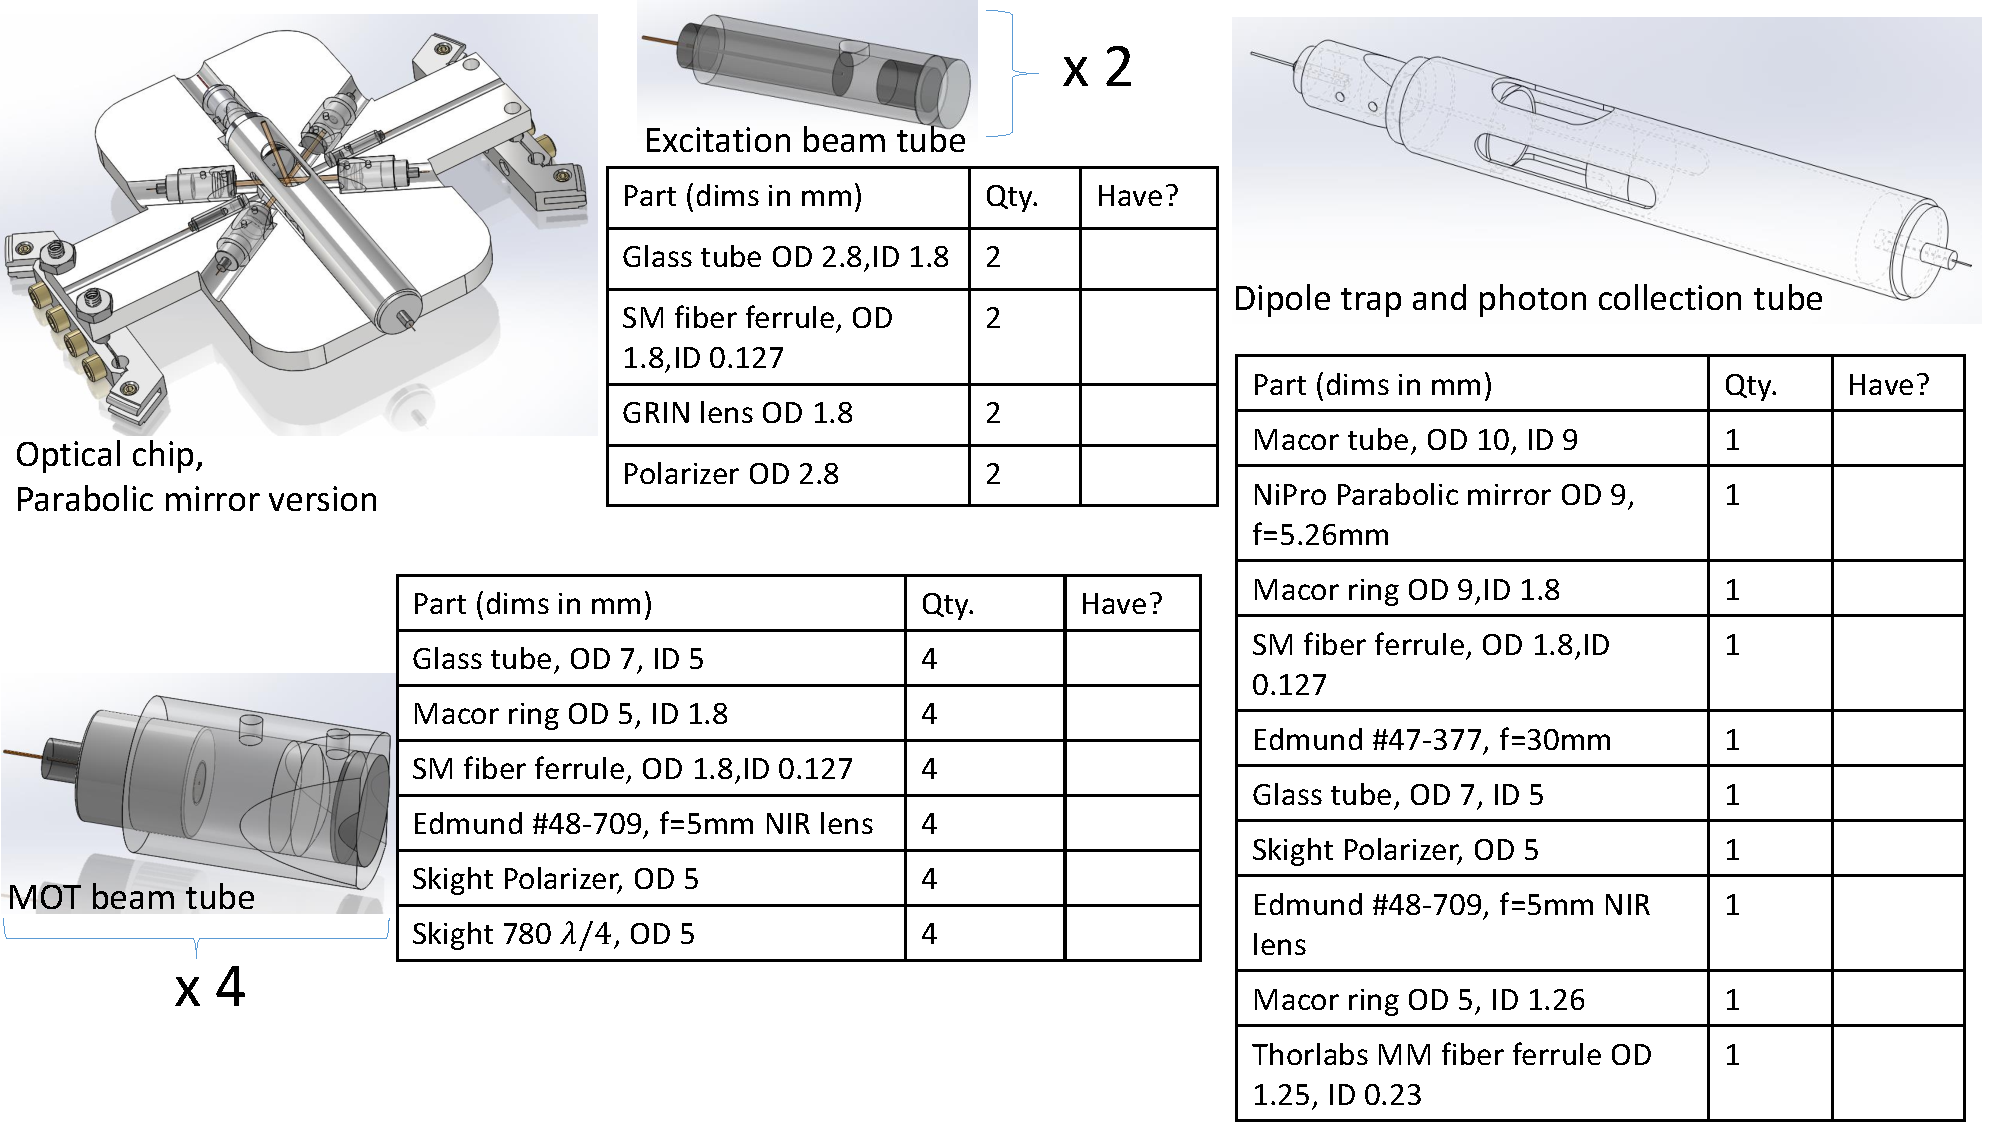
\includegraphics[width=1\textwidth]{Images/optical_chip_parts_mirror_version_20230316.pdf}
    \caption{An ingredients list for the parabolic mirror version of the optical chip which was used in the first network node. The columns labeled ``have?" are so that this sheet can be used to take inventory of the parts we have on hand. In the upper right, the parabolic mirror tube is drawn as being transparent only for the purpose of making the internal contents visible.}.
    \label{fig:mirror_chip_ingredients}
\end{sidewaysfigure}

\newpage